\section{Impact of fingerprinting on Machine Learning models}\label{sec:Learning}
In this section, we evaluate the utility of fingerprinted datasets by measuring the difference in the performance of classifiers for a predictive task, using the original and the fingerprinted dataset. 
We use \textit{accuracy} and \textit{F1} as performance measures. 
In Machine Learning, binary classification is the task of classifying the elements of a given set into two groups (also, categories or classes). 
Given a classification of a specific data set, there are four basic combinations of the actual data class and the assigned class: true positives (TP; actual positive and predicted positive), false positives (FP; actual negative and predicted positive), true negatives (TN; actual negative and predicted negative) and false negatives (FN; actual positive and predicted negative), where "positive" and "negative" represent two classes. 
These combinations can be arranged into a 2x2 contingency table as shown in \Cref{fig:confusion-matrix-binary}.

\begin{figure}
    \centering
    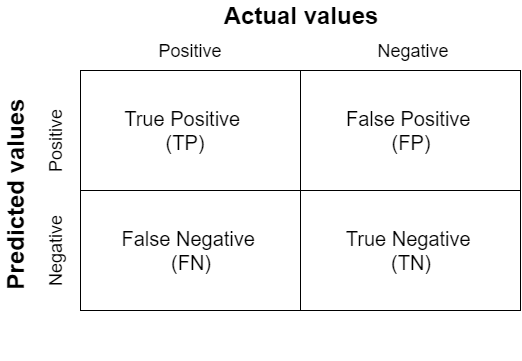
\includegraphics[width=0.6\textwidth]{Figures/confusion.png}
    \caption{Combinations of actual data classes and assigned classes in binary classification}
    \label{fig:confusion-matrix-binary}
\end{figure}

A calculation of the classification accuracy and F1 score is based on a number of occurrences of each combination in the classification. 
Accuracy is the ratio of a number of correct predictions to the total number of input samples.
Accuracy of a binary classification is defined as:
\begin{equation}\label{eq:accuracy-binary}
    accuracy = \frac{TP+TN}{P+N}
\end{equation}
where $P = TP+FP$ and $N = TN+FN$.
F1 score of binary classification is the harmonic average of the precision and the recall.
Precision, recall and F1 score for the binary classification are defined as follows:
\begin{equation}
    precision = \frac{TP}{TP+FP}
\end{equation}
\begin{equation}
    recall = \frac{TP}{TP+FN}
\end{equation}
\begin{equation}\label{eq:f1-binary}
    F1 = 2 \cdot \frac{precision \cdot recall}{precision + recall}
\end{equation}

The metrics are shown graphically in \Cref{fig:performance-metrics}.

\begin{figure}
    \centering
    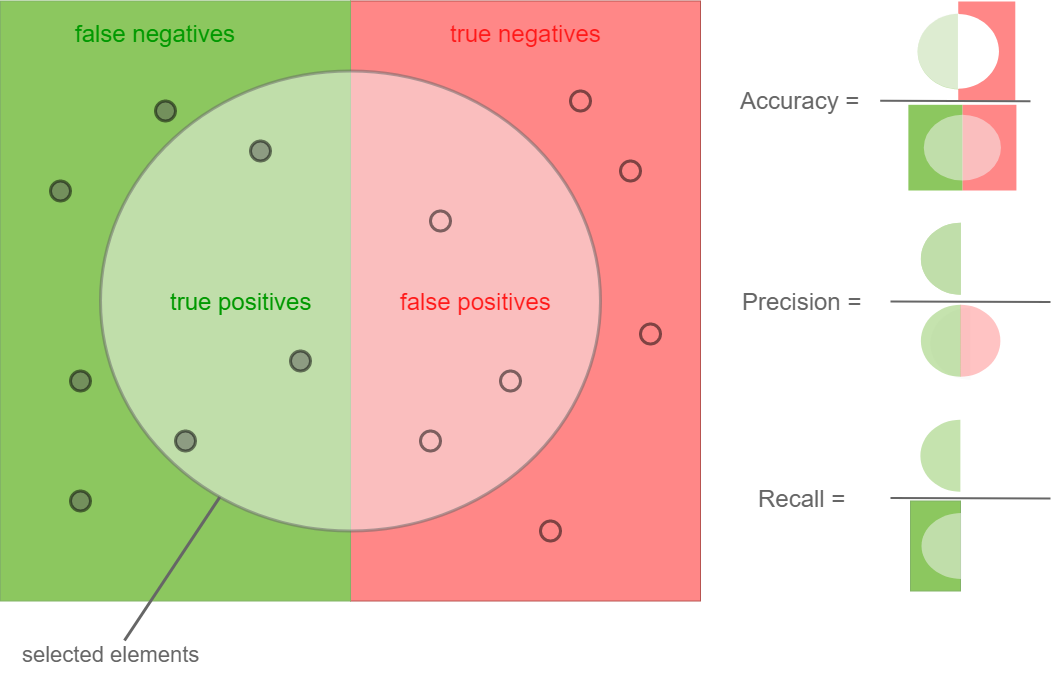
\includegraphics[width=0.8\textwidth]{Figures/metrics.png}
    \caption{Classification performance metrics}
    \label{fig:performance-metrics}
\end{figure}

Multiclass (or multinomial) classification is the task of classifying the elements of a given set into three or more groups (categories, classes). 
It can be denoted as a function $g(x)$ that on input $x$ returns one of the classes ${1,...,K}$.
Similarly to the binary classification, we can distinguish the combinations of actual data class and the predicted one. In this case, we have true positives, false positives and false negatives associated with each class $i$.
$\text{TP}_i$ denotes the instances from the class $i$ that are predicted to be in the class $i$, $\text{FP}_i$ are instances belonging to another class, falsely predicted to be in the class $i$, and $\text{FN}_i$ are the instances from the class $i$ falsely predicted to be in some other class. 

The accuracy of the multinomial classification is calculated as:
\begin{equation}\label{eq:accuracy-multiclass}
    accuracy = \frac{1}{\eta}\cdot \sum_{i=1}^{K}\text{TP}_i
\end{equation}
where $\eta$ is a total number of data instances. Note that \Cref{eq:accuracy-multiclass} is the general form that applies to the binary classification as well. 

For multiclass classification, precision and recall can be micro- or macro-averaged, therefore also can be F1 score.
The micro-averaged precision and recall are defined as follows:
\begin{equation}
    precision_{micro} = \frac{\sum_{i=1}^{K}\text{TP}_i}{\sum_{i=1}^{K}\text{TP}_i + \text{FP}_i}
\end{equation}
\begin{equation}
    recall_{micro} = \frac{\sum_{i=1}^{K}\text{TP}_i}{\sum_{i=1}^{K}\text{TP}_i + \text{FN}_i}
\end{equation}
Therefore, the micro F1 score is: 
\begin{equation}
    F1_{micro} = 2 \cdot \frac{precision_{micro} \cdot recall_{micro}}{precision_{micro} + recall_{micro}}
\end{equation}
If micro F1 is a large value, this indicates that a classifier performs well overall, however it is not sensitive to the performance of individual classes. 
The macro-averaged precision and recall are:
\begin{equation}
    precision_{macro} = \frac{1}{K}\sum_{i=1}^{K}\frac{\text{TP}_i}{\text{TP}_i + \text{FP}_i}
\end{equation}
\begin{equation}
    recall_{macro} = \frac{1}{K}\sum_{i=1}^{K}\frac{\text{TP}_i}{\text{TP}_i + \text{FN}_i}
\end{equation}
Hence, the macro F1 score is:
\begin{equation}\label{eq:f1-macro}
    F1_{macro} = 2 \cdot \frac{precision_{macro} \cdot recall_{macro}}{precision_{macro} + recall_{macro}}
\end{equation}
A large macro F1 suggests that the classifier performs well for each individual class. The macro-average is therefore more suitable for data with an imbalanced class distribution.
All of the above metrics reach their best value at 1 for the perfect classifier and worst at 0.

\paragraph{Experimental setup}
We used three datasets for the experiments - the Forest dataset, the Adult dataset and the Credit dataset. Therefore, three different classifications have been analysed. 
In the Forest dataset, the target attribute is \textit{covertype} with 7 values, thus we are solving the multiclass classification problem. 
The accuracy is calculated as in \Cref{eq:accuracy-multiclass}. Furthermore, we choose to use macro averages for calculating the F1 score (\Cref{eq:f1-macro}) to avoid the misleading nature of micro averages when the class distribution is imbalanced.

In the Adult dataset, we are predicting the binary attribute \textit{income}. In the German Credit dataset, we are as well predicting the binary target attribute that classifies the data instance as good or bad credit risk. The binary classification is being performed and analysed for these two datasets and accordingly, the classification accuracy and F1 are calculated as \Cref{eq:accuracy-binary} and \Cref{eq:f1-binary}.

For all of our experiments, we use 10-fold cross-validation to evaluate Machine Learning models.
$k$-fold cross-validation is a resampling procedure used in Machine Learning to estimate the skill of a Machine Learning model on unseen data.
It generally results in a less biased or less optimistic estimate of the model skill than other methods, such as a simple train/test split. 
The procedure starts by shuffling the dataset randomly and splitting it into $k$ groups. In our experiments $k=10$. 
Each unique group is taken as a hold out (test dataset) while the remaining $k-1$ groups are taken as a training dataset.
It fits a model on the training set and evaluates it on the test set, retaining the evaluation score for that group.
At the end, we summarise the skill of the model using the sample of model evaluation scores.
In the experiments, we record the average of these scores. 

Generally, the goal was not to build models with best predictions but to compare the effectiveness of the fingerprinted data compared to the original.
Therefore, there is no advanced parameter optimisation included nor we dive into more complicated feature selection for building models, as it would shift the focus from the main goal. 
Still, we wanted to achieve the model performance levels rather close to the benchmark solutions available from numerous online sources\footnote{\url{https://www.kaggle.com/wenruliu/adult-income-dataset/kernels}}\footnote{\url{https://www.kaggle.com/c/forest-cover-type-prediction/kernels}} (the chosen datasets and the correlated classification problems are well known in the Machine Learning community).
Therefore, it was important to find good hyperparameters for each of the classification tasks and each classifier.
One possible solution besides the pure manual tuning is a random search over hyperparameters.
We set up a grid of hyperparameter values and select a limited number of random combinations to train the model and score on validations data.
This way we choose the combination of parameters giving the best score for our model.

We use Randomized Search with 10 iterations from the Python scikit-learn package\footnote{\url{https://scikit-learn.org/stable/}} for tuning most important hyperparameters. 
Evaluation within the random search is done using 10-fold cross-validation and F1 score (macro F1 in case of a multiclass classification). 

Finally, for our experiments, we use the following classifiers, all implemented in the Python scikit-learn package:
\begin{itemize}
    \item Decision Tree
    \item k-NN (k Nearest Neighbours)
    \item Logistic regression
    \item Random Forest
    \item Gradient Boosting
\end{itemize}

The experimental process in the following sections has the following steps:
\begin{enumerate}
    \item Use random search to tune the hyperparameters of the Decision Tree, k-NN, Logistic Regression, Random Forest and Gradient Boosting classifiers. In some of the experiments, we use only the subset of the classifiers above. 
    \item Train the model with the original dataset and score the classification accuracy and F1
    \item For each fingerprinting parameter combination $(\gamma, \xi)$ train the model with the fingerprinted dataset and score the classification accuracy and F1. Set the hyperparameters according to step 1.  
    \item Record the differences in the performance measures
    \item Steps 3 and 4 are repeated 10 times to get the average values. In every experiment, we fingerprint the data with a random choice of buyer's id and secret key.
    
\end{enumerate}


% Forest dataset
\subsection{Forest Cover Type}
The first set of experiments is made using the biggest of the three datasets - Forest Cover Type. 
We use the AK Scheme for fingerprinting the numerical attributes of the dataset.
The target attribute is \textit{covertype} and all the others are used as an input for a prediction. 
We use the following classifiers and set the following hyperparameters:
    \begin{itemize}
        \item Decision Tree: $max\_depth=5$, $criterion=entropy$
        \item Logistic Regression: $C=100$
        \item Random Forest: $n\_estimators=100$
    \end{itemize}
    The other hyperparameters are set to default values from the scikit-learn implementations of the classifiers.

The average differences are shown in \Cref{tab:dt_forest_diff,tab:lr_forest_diff,tab:rf_forest_diff} for Decision Tree, Logistic Regression and Random Forest, respectively.

\begin{table}[ht]
    \centering
    \caption{Effects on F1 score and classification accuracy of a Decision Tree model trained with the Forest Cover Type dataset}
    \label{tab:dt_forest_diff}
    \resizebox{\textwidth}{!}{
    \begin{tabular}{|l|rr|rr|rr||rr|}
    \hline
        &  \multicolumn{2}{c|}{$\xi=2$} &  \multicolumn{2}{c|}{$\xi=4$} &  \multicolumn{2}{c||}{$\xi=6$} & 
        \multicolumn{2}{c|}{average} \\
        & F1 & acc. & F1 & acc.  & F1 & acc. & F1 & acc. \\
        \hline
         $\gamma=100$ & 0\% & 0\% & 0\% & \textcolor{red}{-0.01\%} & 0\% & \textcolor{red}{-0.01\%} & 0\% & \textcolor{red}{-0.01\%}\\
         \hline
         $\gamma=50$ & 0\% & \textcolor{red}{-0.02\%} & 0\% & 0\% & 0\% & +0.01\% & 0\% & 0\%\\
         \hline
         $\gamma=25$ & 0\% & \textcolor{red}{-0.02\%} & +0.02\% & +0.01\% & \textcolor{red}{-0.03\%} & \textcolor{red}{-0.01\%} & 0\% & \textcolor{red}{-0.01\%}\\
         \hline
         $\gamma=12$ & \textcolor{red}{-0.01\%} & \textcolor{red}{-0.02\%} & \textcolor{red}{-0.01\%} & 0\% & \textcolor{red}{-0.01\%} & \textcolor{red}{-0.10\%} & \textcolor{red}{-0.01\%} & \textcolor{red}{-0.04\%}\\
         \hline
         $\gamma=6$ & \textcolor{red}{-0.01\%} & 0\% & \textcolor{red}{-0.04\%} & \textcolor{red}{-0.01\%} & \textcolor{red}{-0.19\%} & \textcolor{red}{-0.11\%} & \textcolor{red}{-0.08\%} & \textcolor{red}{-0.04\%}\\
         \hline
         \hline
         average & 0\% & \textcolor{red}{-0.1\%} & \textcolor{red}{-0.01\%} & 0\% & \textcolor{red}{-0.05\%} & \textcolor{red}{-0.04\%} & \textbf{\textcolor{red}{-0.07\%}} & \textbf{\textcolor{red}{-0.02\%}}\\
         \hline
    \end{tabular}}
\end{table}


\begin{table}[ht]
    \centering
    \caption{Effects on F1 score and classification accuracy of a Logistic Regression model trained with the Forest Cover Type dataset}
    \label{tab:lr_forest_diff}
    \resizebox{\textwidth}{!}{
    \begin{tabular}{|l|rr|rr|rr||rr|}
    \hline
        &  \multicolumn{2}{c|}{$\xi=2$} &  \multicolumn{2}{c|}{$\xi=4$} &  \multicolumn{2}{c||}{$\xi=6$} & 
        \multicolumn{2}{c|}{average} \\
        & F1 & acc. & F1 & acc. & F1 & acc. & F1 & acc. \\
        \hline
         $\gamma=100$  & 0\% & 0\% & +0.01\% & 0\% & \textcolor{red}{-0.01\%} & +0.01\% & 0\% & 0\%\\
         \hline
         $\gamma=50$ & \textcolor{red}{-0.02\%} & 0\% & +0.01\% & 0\% & \textcolor{red}{-0.01\%} & +0.01\% & \textcolor{red}{-0.01\%} & 0\% \\
         \hline
         $\gamma=25$  & 0\% & 0\% & \textcolor{red}{-0.01\%} & \textcolor{red}{-0.01\%} & \textcolor{red}{-0.05\%} & +0.02\% & \textcolor{red}{-0.02\%} & 0\%\\
         \hline
         $\gamma=12$  & 0\% & 0\% & \textcolor{red}{-0.02\%} & 0\% & \textcolor{red}{-0.11\%} & +0.02\% & \textcolor{red}{-0.04\%} & 0\%\\
         \hline
         $\gamma=6$  & 0\% & 0\% & \textcolor{red}{-0.03\%} & 0\% & \textcolor{red}{-0.14\%} & +0.03\% & \textcolor{red}{-0.06\%} & +0.01\% \\
         \hline
         \hline
         average & 0\% & 0\% & \textcolor{red}{-0.01\%} & 0\% & \textcolor{red}{-0.07\%} & +0.02\% & \textbf{\textcolor{red}{-0.03\%}} & \textbf{+0.01\%}\\
         \hline
    \end{tabular}}
\end{table}


\begin{table}[ht]
    \centering
    \caption{Effects on F1 score and classification accuracy of a Random Forest model trained with the Forest Cover Type dataset}
    \label{tab:rf_forest_diff}
    \resizebox{\textwidth}{!}{
    \begin{tabular}{|l|rr|rr|rr||rr|}
    \hline
        &  \multicolumn{2}{c|}{$\xi=2$} &  \multicolumn{2}{c|}{$\xi=4$} &  \multicolumn{2}{c||}{$\xi=6$} & \multicolumn{2}{c|}{average} \\
        & F1 & acc. & F1 & acc. & F1 & acc. & F1 & acc. \\
        \hline
         $\gamma=100$ & +0.01\% & \textcolor{red}{-0.03\%} & +0.01\% & \textcolor{red}{-0.05\%} & \textcolor{red}{-0.06\%} & \textcolor{red}{-0.08\%} & \textcolor{red}{-0.01\%} & \textcolor{red}{-0.05\%} \\

         \hline
         $\gamma=50$  & 0\% & 0\% & +0.01\% & +0.02\% & \textcolor{red}{-0.02\%} & \textcolor{red}{-0.03\%} & 0\% & 0\% \\ 
    
        \hline
         $\gamma=25$  & 0\% & \textcolor{red}{-0.01\%} & \textcolor{red}{-0.07\%} & \textcolor{red}{-0.03\%} & \textcolor{red}{-0.05\%} & \textcolor{red}{-0.03\%} & \textcolor{red}{-0.04\%} & \textcolor{red}{-0.02\%} \\ 
         
        \hline
         $\gamma=12$  & \textcolor{red}{-0.02\%} & 0\% & \textcolor{red}{-0.01\%} & 0\% & \textcolor{red}{-0.03\%} & \textcolor{red}{-0.05\%} & \textcolor{red}{-0.02\%} & \textcolor{red}{-0.02\%}\\ 

        \hline
         $\gamma=6$  & \textcolor{red}{-0.04\%} & \textcolor{red}{-0.08\%} & \textcolor{red}{-0.01\%} & \textcolor{red}{-0.03\%} & 0\% & \textcolor{red}{-0.01\%} & \textcolor{red}{-0.02\%} & \textcolor{red}{-0.04\%}\\ 
      
        \hline
        \hline
        average & \textcolor{red}{-0.01\%} & \textcolor{red}{-0.03\%} & \textcolor{red}{-0.01\%} & \textcolor{red}{-0.02\%} & \textcolor{red}{-0.03\%} & \textcolor{red}{-0.04\%} & \textbf{\textcolor{red}{-0.02\%}} & \textbf{\textcolor{red}{-0.03\%}} \\
        \hline
    \end{tabular}}
\end{table}

The changes in performance are generally very small (in most of the cases the difference is in the 4th decimal place of the absolute values), therefore we represent the changes as percentages in range (0-100\%). 
All of the results roughly follow the rule that the performance measures decrease when $\gamma$ decreases, i.e. more marks introduced in data. We can observe this behaviour in the last columns of every table where we calculate the average F1 score and accuracy for a fixed $\gamma$ 
Furthermore, a general rule holds that the performance slightly drops for larger $\xi$ values, i.e. more bits available for fingerprinting. This is due to larger distortions of particular values in the data.
This is shown in the last row of every table where we average out the F1 score and accuracy for a fixed $\xi$.
Every classifier from the experiments behaves very similarly in the means of performance decrease. Overall average F1 score and accuracy for every classifier is calculated from the experiment results and presented the bottom rightmost cell of each table. 

On the Forest Cover Type data, we can conclude that the differences observed when using the Decision Tree classifier (see \Cref{tab:dt_forest_diff}) are rather minute, and would not constitute a noticeable degradation of effectiveness. 
The trend is the same also for other classifiers, as can be seen in \Cref{tab:lr_forest_diff} for Logistic Regression, and \Cref{tab:rf_forest_diff} for Random Forest.
In a few cases, the classification results obtained even improved, for example, the accuracy of Logistic Regression trained by data fingerprinted using $\xi=6$, though by the same rather marginal order of magnitude as the observed decline. 



% Adult data
\subsection{Adult (Census Data)}
We make the set of experiments using the Adult dataset. The dataset is mostly composed of categorical values, thus we use the fingerprinting scheme for categorical data from \Cref{subsec:fingerprinting-scheme-categorical}.
The target of the classification task is \textit{income}.
All other attributes (including numerical, although we do not fingerprint them) are used for as an input for a classifier.
We use Decision Tree, k-NN, Logistic Regression and Gradient Boosting. The hyperparameters are set as follows:
    \begin{itemize}
        \item k-NN: $n\_neighbors=19$
        \item Logistic Regression: $solver=liblinear$, $C=20$
        \item Random Forest: $n\_estimators=200$, $max\_depth=15$, $criterion=gini$
        \item Gradient Boosting: $n\_estimators:=40$, $max\_depth=8$, $loss=deviance$, $criterion=mse$
    \end{itemize}

The differences in F1 and accuracy scores (on a scale $[0,100]\%$) between original and fingerprinted Adult dataset for Decision Tree, k-NN, Logistic Regression, Random Forest and Gradient Boosting are shown in \Cref{tab:knn_adult_diff,tab:lr_adult_diff,tab:rf_adult_diff,tab:gb_adult_diff}.

\begin{table}[ht]
    \centering
    \caption{Effects on F1 score and classification accuracy of a k-NN model trained with the Adult dataset}
    \label{tab:knn_adult_diff}
    \resizebox{\textwidth}{!}{
    \begin{tabular}{|c|rr|rr|rr|rr||rr|}
    \hline
        & \multicolumn{2}{c|}{$\xi=1$} &  \multicolumn{2}{c|}{$\xi=2$} &  \multicolumn{2}{c|}{$\xi=4$} &  \multicolumn{2}{c||}{$\xi=6$} &  \multicolumn{2}{c|}{average} \\
        & F1 & acc. & F1 & acc. & F1 & acc. & F1 & acc. & F1 & acc.\\
        \hline
         $\gamma=50$ & +0.05\% & +0.03\% & \textcolor{red}{-0.10\%} & \textcolor{red}{-0.05\%} & \textcolor{red}{-0.06\%} & \textcolor{red}{-0.02\%} & \textcolor{red}{-0.02\%} & +0.01\% & \textcolor{red}{-0.03\%} & \textcolor{red}{-0.01\%}\\
         \hline
         $\gamma=25$ & \textcolor{red}{-0.10\%} & \textcolor{red}{-0.05\%} & +0.05\% & +0.02\% & +0.07\% & +0.03\% & \textcolor{red}{-0.02\%} & +0.03\% & 0\% & \textcolor{red}{-0.01\%} \\
         \hline
         $\gamma=12$ & \textcolor{red}{-0.32\%} & \textcolor{red}{-0.19\%} & \textcolor{red}{-0.10\%} & \textcolor{red}{-0.06\%} & +0.02\% & +0.03\% & \textcolor{red}{-0.20\%} & \textcolor{red}{-0.04\%} & \textcolor{red}{-0.15\%} & \textcolor{red}{-0.07\%}\\
         \hline
         $\gamma=6$ & \textcolor{red}{-0.70\%} & \textcolor{red}{-0.42\%} & \textcolor{red}{-0.50\%} & \textcolor{red}{-0.22\%} & \textcolor{red}{-0.36\%} & \textcolor{red}{-0.15\%} & \textcolor{red}{-0.60\%} & \textcolor{red}{-0.21\%} & \textcolor{red}{-0.54\%} & \textcolor{red}{-0.25\%}\\
         \hline
         $\gamma=3$ & \textcolor{red}{-1.79\%} & \textcolor{red}{-1.02\%} & \textcolor{red}{-0.70\%} & \textcolor{red}{-0.36\%} & \textcolor{red}{-0.61\%} & \textcolor{red}{-0.22\%} & \textcolor{red}{-0.81\%} & \textcolor{red}{-0.32\%} & \textcolor{red}{-0.98\%} & \textcolor{red}{-0.48\%}\\
         \hline
         \hline
         average & \textcolor{red}{-0.57\%} & \textcolor{red}{-0.33\%} & \textcolor{red}{-0.27\%} & \textcolor{red}{-0.13\%} & \textcolor{red}{-0.19\%} & \textcolor{red}{-0.07\%} & \textcolor{red}{-0.33\%} & \textcolor{red}{-0.11\%} & \textbf{\textcolor{red}{-0.34\%}} & \textbf{\textcolor{red}{-0.16\%}}  \\
         \hline
    \end{tabular}}
\end{table}


\begin{table}[ht]
    \centering
    \caption{Effects on F1 score and classification accuracy of a Logistic Regression model trained with the Adult dataset}
    \label{tab:lr_adult_diff}
    \resizebox{\textwidth}{!}{
    \begin{tabular}{|c|rr|rr|rr|rr||rr|}
    \hline
        & \multicolumn{2}{c|}{$\xi=1$} &  \multicolumn{2}{c|}{$\xi=2$} &  \multicolumn{2}{c|}{$\xi=4$} &  \multicolumn{2}{c||}{$\xi=6$} & 
        \multicolumn{2}{c|}{average}\\
        & F1 & acc. & F1 & acc. & F1 & acc. & F1 & acc. & F1 & acc. \\
        \hline
         $\gamma=50$ & \textcolor{red}{-0.15\%} & \textcolor{red}{-0.07\%} & \textcolor{red}{-0.02\%} & \textcolor{red}{-0.01\%} & \textcolor{red}{-0.07\%} & \textcolor{red}{-0.03\%} & \textcolor{red}{-0.03\%} & \textcolor{red}{-0.02\%} & \textcolor{red}{-0.07\%} & \textcolor{red}{-0.03\%}\\
        \hline
         $\gamma=25$ & \textcolor{red}{-0.25\%} & \textcolor{red}{-0.14\%} & \textcolor{red}{-0.13\%} & \textcolor{red}{-0.06\%} & \textcolor{red}{-0.10\%} & \textcolor{red}{-0.06\%} & \textcolor{red}{-0.14\%} & \textcolor{red}{-0.06\%} & \textcolor{red}{-0.16\%} & \textcolor{red}{-0.08\%}\\
        \hline
         $\gamma=12$ & \textcolor{red}{-0.46\%} & \textcolor{red}{-0.22\%} & \textcolor{red}{-0.27\%} & \textcolor{red}{-0.12\%} & \textcolor{red}{-0.12\%} & \textcolor{red}{-0.08\%} & \textcolor{red}{-0.39\%} & \textcolor{red}{-0.15\%} & \textcolor{red}{-0.31\%} & \textcolor{red}{-0.14\%}\\
        \hline
         $\gamma=6$ & \textcolor{red}{-0.68\%} & \textcolor{red}{-0.38\%} & \textcolor{red}{-0.41\%} & \textcolor{red}{-0.22\%} & \textcolor{red}{-0.46\%} & \textcolor{red}{-0.19\%} & \textcolor{red}{-0.80\%} & \textcolor{red}{-0.33\%} & \textcolor{red}{-0.59\%} & \textcolor{red}{-0.28\%}\\
        \hline
         $\gamma=3$ & \textcolor{red}{-2.12\%} & \textcolor{red}{-1.01\%} & \textcolor{red}{-1.08\%} & \textcolor{red}{-0.52\%} & \textcolor{red}{-0.75\%} & \textcolor{red}{-0.32\%} & \textcolor{red}{-1.33\%} & \textcolor{red}{-0.62\%} & \textcolor{red}{-1.32\%} & \textcolor{red}{-0.62\%}\\
        \hline
        \hline
        average & \textcolor{red}{-0.73\%} & \textcolor{red}{-0.36\%} & \textcolor{red}{-0.38\%} & \textcolor{red}{-0.19\%} & \textcolor{red}{-0.25\%} & \textcolor{red}{-0.14\%} & \textcolor{red}{-0.54\%} & \textcolor{red}{-0.24\%} & \textbf{\textcolor{red}{-0.49\%}} & \textbf{\textcolor{red}{-0.23\%}} \\
        \hline
    \end{tabular}}
\end{table}


\begin{table}[ht]
    \centering
    \caption{Effects on F1 score and classification accuracy of a Random Forest model trained with the Adult dataset}
    \label{tab:rf_adult_diff}
    \resizebox{\textwidth}{!}{
    \begin{tabular}{|c|rr|rr|rr|rr||rr|}
    \hline
        & \multicolumn{2}{c|}{$\xi=1$} &  \multicolumn{2}{c|}{$\xi=2$} &  \multicolumn{2}{c|}{$\xi=4$} &  \multicolumn{2}{c||}{$\xi=6$} & \multicolumn{2}{c|}{average}\\
        & F1 & acc. & F1 & acc. & F1 & acc. & F1 & acc. & F1 & acc. \\
        \hline
         $\gamma=50$  & \textcolor{red}{-0.04\%} & +0.06\% & \textcolor{red}{-0.40\%} & \textcolor{red}{-0.10\%} & \textcolor{red}{-0.02\%} & +0.02\% & \textcolor{red}{-0.37\%} & \textcolor{red}{-0.09\%} & \textcolor{red}{-0.21\%} & \textcolor{red}{-0.03\%}\\
        \hline
         $\gamma=25$ & \textcolor{red}{-0.28\%} & \textcolor{red}{-0.13\%} & \textcolor{red}{-0.20\%} & \textcolor{red}{-0.03\%} & \textcolor{red}{-0.29\%} & \textcolor{red}{-0.08\%} & \textcolor{red}{-0.56\%} & \textcolor{red}{-0.15\%} & 
         \textcolor{red}{-0.33\%} & \textcolor{red}{-0.10\%} \\
        \hline
         $\gamma=12$ & \textcolor{red}{-0.59\%} & \textcolor{red}{-0.23\%} & \textcolor{red}{-0.63\%} & \textcolor{red}{-0.23\%} & \textcolor{red}{-0.13\%} & +0.02\% & \textcolor{red}{-0.34\%} & \textcolor{red}{-0.09\%} & \textcolor{red}{-0.42\%} & \textcolor{red}{-0.13\%}\\
        \hline
         $\gamma=6$ & \textcolor{red}{-0.68\%} & \textcolor{red}{-0.31\%} & \textcolor{red}{-0.66\%} & \textcolor{red}{-0.20\%} & \textcolor{red}{-0.33\%} & \textcolor{red}{-0.08\%} & \textcolor{red}{-0.76\%} & \textcolor{red}{-0.24\%} & \textcolor{red}{-0.61\%} & \textcolor{red}{-0.27\%}\\
        \hline
         $\gamma=3$ & \textcolor{red}{-2.26\%} & \textcolor{red}{-1.02\%} & \textcolor{red}{-1.04\%} & \textcolor{red}{-0.37\%} & \textcolor{red}{-1.24\%} & \textcolor{red}{-0.40\%} & \textcolor{red}{-1.01\%} & \textcolor{red}{-0.35\%} & \textcolor{red}{-1.39\%} & \textcolor{red}{-0.54\%}\\
        \hline
        \hline
        average & \textcolor{red}{-0.77\%} & \textcolor{red}{-0.33\%} & \textcolor{red}{-0.59\%} & \textcolor{red}{-0.19\%} & \textcolor{red}{-0.40\%} & \textcolor{red}{-0.10\%} & \textcolor{red}{-0.61\%} & \textcolor{red}{-0.18\%} & \textbf{\textcolor{red}{-0.69\%}} & \textbf{\textcolor{red}{-0.20\%}} \\
        \hline
    \end{tabular}}
\end{table}



\begin{table}[ht]
    \centering
    \caption{Effects on F1 score and classification accuracy of a Gradient Boosting model trained with the Adult dataset}
    \label{tab:gb_adult_diff}
    \resizebox{\textwidth}{!}{
    \begin{tabular}{|c|rr|rr|rr|rr||rr|}
    \hline
        & \multicolumn{2}{c|}{$\xi=1$} &  \multicolumn{2}{c|}{$\xi=2$} &  \multicolumn{2}{c|}{$\xi=4$} &  \multicolumn{2}{c||}{$\xi=6$} & \multicolumn{2}{c|}{average} \\
        & F1 & acc. & F1 & acc. & F1 & acc. & F1 & acc. & F1 & acc.\\
        \hline
         $\gamma=50$ & \textcolor{red}{-0.12\%} & \textcolor{red}{-0.06\%} & \textcolor{red}{-0.32\%} & \textcolor{red}{-0.16\%} & +0.02\% & \textcolor{red}{-0.01\%} & \textcolor{red}{-0.17\%} & \textcolor{red}{-0.07\%} &
         \textcolor{red}{-0.15\%} & \textcolor{red}{-0.08\%}\\
         \hline 
         $\gamma=25$ & \textcolor{red}{-0.40\%} & \textcolor{red}{-0.19\%} & \textcolor{red}{-0.43\%} & \textcolor{red}{-0.20\%} & \textcolor{red}{-0.13\%} & \textcolor{red}{-0.08\%} & \textcolor{red}{-0.30\%} & \textcolor{red}{-0.10\%} &
         \textcolor{red}{-0.32\%} & \textcolor{red}{-0.14\%}\\
         \hline 
         $\gamma=12$ & \textcolor{red}{-0.71\%} & \textcolor{red}{-0.34\%} & \textcolor{red}{-0.51\%} & \textcolor{red}{-0.18\%} & \textcolor{red}{-0.42\%} & \textcolor{red}{-0.18\%} & \textcolor{red}{-0.29\%} & \textcolor{red}{-0.11\%} &
         \textcolor{red}{-0.48\%} & \textcolor{red}{-0.20\%}\\
         \hline 
         $\gamma=6$ & \textcolor{red}{-0.85\%} & \textcolor{red}{-0.45\%} & \textcolor{red}{-0.74\%} & \textcolor{red}{-0.35\%} & \textcolor{red}{-0.39\%} & \textcolor{red}{-0.20\%} & \textcolor{red}{-0.69\%} & \textcolor{red}{-0.30\%} &
         \textcolor{red}{-0.67\%} & \textcolor{red}{-0.33\%}\\
         \hline 
         $\gamma=3$ & \textcolor{red}{-2.60\%} & \textcolor{red}{-1.22\%} & \textcolor{red}{-1.18\%} & \textcolor{red}{-0.59\%} & \textcolor{red}{-0.76\%} & \textcolor{red}{-0.36\%} & \textcolor{red}{-0.59\%} & \textcolor{red}{-0.27\%} & 
         \textcolor{red}{-1.28\%} & \textcolor{red}{-0.61\%} \\
         \hline
         \hline
         average & \textcolor{red}{-0.94\%} & \textcolor{red}{-0.45\%} & \textcolor{red}{-0.64\%} & \textcolor{red}{-0.30\%} & \textcolor{red}{-0.34\%} & \textcolor{red}{-0.17\%} & \textcolor{red}{-0.41\%} & \textcolor{red}{-0.17\%} & \textbf{\textcolor{red}{-0.58\%}} & \textbf{\textcolor{red}{-0.27\%}}\\
         \hline
    \end{tabular}}
\end{table}

Overall, each classifier shows a decrease in performance when the fingerprint is applied. 
Except for a few cases where the performance slightly improves, both F1 and accuracy decrease up to approximately 2\%. 
The average difference for each classifier can be seen in the respective table in the rightmost cell of the last row in bold characters. 
The largest average difference for the entire classifier is the change in F1 score of Gradient Boosting, -0.58\% (\Cref{tab:gb_adult_diff}). Therefore, we can argue that changes in F1 and accuracy in this range are rather acceptable. This is, of course, dependable on the use case. However, we need to consider that fingerprinting necessarily changes the values in the dataset and the performance can not be exactly the same as when the original dataset is used. 
The occurrences of the positive differences (see, for example, \Cref{tab:lr_adult_diff}, $\gamma=50$, $\xi=1$) are random and minute, and therefore concluding that a fingerprint in the data improves the performance of the Machine Learning model is a rule for certain cases would be wrong.

In the last row and the last column of every table, we calculate the average difference for the fixed $\xi$ or $\gamma$, respectively, to see the effects of these parameters more easily.
It is hard to detect any pattern between average values of F1/accuracy and $\xi$ value for any of the classifiers. 
This behaviour can be expected because bigger $\xi$ do not imply "more change" in values for this fingerprinting scheme compared to the schemes for numerical values.
For instance, using $\xi=3$ in fingerprinting could change a value "9" to "13" (difference of 4), while using $\xi=1$ could only (and at most!) change it to "8" (difference of 1). 
This behaviour does not apply to categorical data since the change from any categorical value to another is unit.
Therefore, the effect of the parameter $\xi$ on the performance of a model trained using fingerprinted data in classification is random. 

On the other hand, we can see the trend of a decrease in performance for smaller values of $\gamma$ in the last column of the tables. Both average F1 and accuracy gradually decrease for smaller $\gamma$, i.e. more marks in the dataset. It is the case for a majority of the particular cases with one fixed value of $\xi$. For example, the entire experimental results with Logistic Regression, in \Cref{tab:lr_adult_diff}, have a perfect inversely proportional relation between a value of $\gamma$ and absolute difference in F1 score or accuracy.

On the Adult dataset we can conclude that, from the classification point of view, the utility of data is preserved after applying the proposed fingerprinting technique for categorical data. The performance drops are not significant and can be controlled by the parameter $\gamma$. 

% German Credit Data
\subsection{German Credit Data}
With the last set of experiments, we analyse the utility of the fingerprinted data that contains a mixture of numerical and non-numerical attributes.
We use the German Credit dataset and apply both AK Scheme to the numerical values and the naive fingerprinting technique for categorical data to non-numerical. 
We unify these two processes into one fingerprinting process since these techniques share the algorithmic steps, except for the modification for marking the categorical values. 
We use Decision Tree, k-NN, Logistic Regression and Random Forest for the classification and follow the usual procedure. We find with the random search that the best hyperparameters for the model trained with original data are as follows:
\begin{itemize}
    \item Decision Tree: $max\_depth=2$, $criterion=entropy$
    \item k-NN: $n\_neighbors=14$
    \item Logistic Regression: $solver=newton-cg$, $C=70$
    \item Random Forest: $n\_estimators=85$, $max\_depth=10$, $criterion=gini$
\end{itemize}

\Cref{tab:dt_german_diff,tab:knn_german_diff,tab:lr_german_diff,tab:rf_german_diff} show the resulting differences in F1 and accuracy scores (on a scale $[0,100]\%$) between original and fingerprinted German Credit data for Decision Tree, k-NN, Logistic Regression and Random Forest, respectively.

\begin{table}[ht]
    \centering
    \caption{Effects on F1 score and classification accuracy of a Decision Tree model trained with the German Credit dataset}
    \label{tab:dt_german_diff}
    \resizebox{\textwidth}{!}{
    \begin{tabular}{|c|rr|rr|rr|rr||rr|}
    \hline
        &  \multicolumn{2}{c|}{$\xi=1$} &  \multicolumn{2}{c|}{$\xi=2$} &  \multicolumn{2}{c|}{$\xi=4$} &  \multicolumn{2}{c||}{$\xi=6$} & \multicolumn{2}{c|}{average}\\
        & F1 & acc. & F1 & acc. & F1 & acc. & F1 & acc. & F1 & acc. \\
        \hline
         $\gamma=12$ & 0\% & 0\% & \textcolor{red}{-0.07\%} & \textcolor{red}{-0.10\%} & \textcolor{red}{-0.07\%} & \textcolor{red}{-0.10\%} & 0\% & 0\% & \textcolor{red}{-0.04\%} & \textcolor{red}{-0.05\%}\\
        \hline
         $\gamma=9$ & 0\% & 0\% & 0\% & 0\% & \textcolor{red}{-0.14\%} & \textcolor{red}{-0.20\%} & \textcolor{red}{-0.14\%} & \textcolor{red}{-0.20\%} & \textcolor{red}{-0.07\%} & \textcolor{red}{-0.10\%}\\
        \hline
         $\gamma=6$ & 0\% & 0\% & \textcolor{red}{-0.07\%} & \textcolor{red}{-0.10\%} & \textcolor{red}{-0.14\%} & \textcolor{red}{-0.20\%} & \textcolor{red}{-0.14\%} & \textcolor{red}{-0.20\%} & \textcolor{red}{-0.09\%} & \textcolor{red}{-0.13\%}\\
        \hline
         $\gamma=3$ & 0\% & 0\% & \textcolor{red}{-0.14\%} & \textcolor{red}{-0.20\%} & \textcolor{red}{-0.14\%} & \textcolor{red}{-0.20\%} & \textcolor{red}{-0.42\%} & \textcolor{red}{-0.60\%} & \textcolor{red}{-0.18\%} & \textcolor{red}{-0.25\%}\\
        \hline
        \hline
    average & 0\% & 0\% & \textcolor{red}{-0.07\%} & \textcolor{red}{-0.10\%} & \textcolor{red}{-0.12\%} & \textcolor{red}{-0.18\%} & \textcolor{red}{-0.18\%} & \textcolor{red}{-0.25\%} & \textbf{\textcolor{red}{-0.09\%}} & \textbf{\textcolor{red}{-0.13\%}} \\
    \hline
    \end{tabular}}
\end{table}


\begin{table}[ht]
    \centering
    
    \caption{Effects on F1 score and classification accuracy of a k-NN model trained with the German Credit dataset}
    \label{tab:knn_german_diff}
    \resizebox{\textwidth}{!}{
    \begin{tabular}{|c|rr|rr|rr|rr||rr|}
    \hline
        &  \multicolumn{2}{c|}{$\xi=1$} &  \multicolumn{2}{c|}{$\xi=2$} &  \multicolumn{2}{c|}{$\xi=4$} &  \multicolumn{2}{c||}{$\xi=6$} & \multicolumn{2}{c|}{average} \\
        & F1 & acc. & F1 & acc. & F1 & acc. & F1 & acc.  & F1 & acc. \\
        \hline
         $\gamma=12$ & 0.0\% & 0.0\% & \textcolor{red}{-0.14\%} & \textcolor{red}{-0.20\%} & \textcolor{red}{-0.07\%} & \textcolor{red}{-0.10\%} & 0.0\% & 0.0\% & \textcolor{red}{-0.05\%} & \textcolor{red}{-0.08\%}\\
        \hline
         $\gamma=9$ & 0.0\% & 0.0\% & \textcolor{red}{-0.05\%} & \textcolor{red}{-0.10\%} & \textcolor{red}{-0.14\%} & \textcolor{red}{-0.20\%} & \textcolor{red}{-0.22\%} & \textcolor{red}{-0.30\%} & \textcolor{red}{-0.10\%} & \textcolor{red}{-0.15\%}\\
        \hline
         $\gamma=6$ & 0.0\% & 0.0\% & \textcolor{red}{-0.27\%} & \textcolor{red}{-0.40\%} & \textcolor{red}{-0.14\%} & \textcolor{red}{-0.20\%} & \textcolor{red}{-0.22\%} & \textcolor{red}{-0.30\%} & \textcolor{red}{-0.16\%} & \textcolor{red}{-0.23\%} \\
        \hline
         $\gamma=3$ & 0.0\% & 0.0\% & \textcolor{red}{-0.09\%} & \textcolor{red}{-0.10\%} & \textcolor{red}{-0.39\%} & \textcolor{red}{-0.60\%} & \textcolor{red}{-0.45\%} & \textcolor{red}{-0.60\%} & \textcolor{red}{-0.23\%} & \textcolor{red}{-0.33\%}\\
        \hline
        \hline
        average & 0\% & 0\% & \textcolor{red}{-0.14\%} & \textcolor{red}{-0.20\%} & \textcolor{red}{-0.19\%} & \textcolor{red}{-0.28\%} & \textcolor{red}{-0.22\%} & \textcolor{red}{-0.30\%} & \textbf{\textcolor{red}{-0.14\%}} & \textbf{\textcolor{red}{-0.19\%}}\\
        \hline
    \end{tabular}}
\end{table}

\begin{table}[ht]
    \centering
    \caption{Effects on F1 score and classification accuracy of a Logistic Regression model trained with the German Credit dataset}
    \label{tab:lr_german_diff}
    \resizebox{\textwidth}{!}{
    \begin{tabular}{|c|rr|rr|rr|rr||rr|}
    \hline
        &  \multicolumn{2}{c|}{$\xi=1$} &  \multicolumn{2}{c|}{$\xi=2$} &  \multicolumn{2}{c|}{$\xi=4$} &  \multicolumn{2}{c||}{$\xi=6$} & \multicolumn{2}{c|}{average} \\
        & F1 & acc. & F1 & acc. & F1 & acc. & F1 & acc. & F1 & acc. \\
        \hline
         $\gamma=12$ & \textcolor{red}{-0.02\%} & 0.0\% & \textcolor{red}{-0.45\%} & \textcolor{red}{-0.61\%} & \textcolor{red}{-0.02\%} & +0.09\% & +0.17\% & +0.30\% & \textcolor{red}{-0.08\%} & \textcolor{red}{-0.06\%} \\ 
         \hline
         $\gamma=9$ & \textcolor{red}{-0.04\%} & 0.0\% & \textcolor{red}{-0.27\%} & \textcolor{red}{-0.30\%} & \textcolor{red}{-0.38\%} & \textcolor{red}{-0.60\%} & \textcolor{red}{-0.25\%} & \textcolor{red}{-0.50\%} & \textcolor{red}{-0.24\%} & \textcolor{red}{-0.35\%}\\
         \hline
         $\gamma=6$ & \textcolor{red}{-0.05\%} & \textcolor{red}{-0.10\%} & \textcolor{red}{-0.42\%} & \textcolor{red}{-0.71\%} & \textcolor{red}{-0.55\%} & \textcolor{red}{-0.80\%} & \textcolor{red}{-0.25\%} & \textcolor{red}{-0.40\%} & \textcolor{red}{-0.32\%} & \textcolor{red}{-0.50\%} \\
        \hline
        $\gamma=3$ & \textcolor{red}{-0.17\%} & \textcolor{red}{-0.30\%} & \textcolor{red}{-0.26\%} & \textcolor{red}{-0.41\%} & \textcolor{red}{-0.21\%} & \textcolor{red}{-0.50\%} & \textcolor{red}{-0.29\%} & \textcolor{red}{-0.41\%} & \textcolor{red}{-0.23\%} & \textcolor{red}{-0.41\%} \\
         \hline
         \hline
         average & \textcolor{red}{-0.07\%} & \textcolor{red}{-0.10\%} & \textcolor{red}{-0.35\%} & \textcolor{red}{-0.51\%} & \textcolor{red}{-0.29\%} & \textcolor{red}{-0.45\%} & \textcolor{red}{-0.16\%} & \textcolor{red}{-0.25\%} & \textbf{\textcolor{red}{-0.22\%}} & \textbf{\textcolor{red}{-0.33\%}}\\
         \hline
    \end{tabular}}
\end{table}


\begin{table}[ht]
    \centering
    \caption{Effects on F1 score and classification accuracy of a decision Tree model trained with the Random Forest dataset}
    \label{tab:rf_german_diff}
    \resizebox{\textwidth}{!}{
    \begin{tabular}{|c|rr|rr|rr|rr||rr|}
    \hline
        &  \multicolumn{2}{c|}{$\xi=1$} &  \multicolumn{2}{c|}{$\xi=2$} &  \multicolumn{2}{c|}{$\xi=4$} &  \multicolumn{2}{c||}{$\xi=6$} & \multicolumn{2}{c|}{average} \\
        & F1 & acc. & F1 & acc. & F1 & acc. & F1 & acc.& F1 & acc. \\
        \hline
         $\gamma=12$ & \textcolor{red}{-0.47\%} & \textcolor{red}{-0.70\%} & \textcolor{red}{-0.81\%} & \textcolor{red}{-1.20\%} & \textcolor{red}{-0.07\%} & \textcolor{red}{-0.31\%} & \textcolor{red}{-0.21\%} & \textcolor{red}{-0.50\%} & \textcolor{red}{-0.39\%} & \textcolor{red}{-0.68\%}\\
        \hline
         $\gamma=9$ & \textcolor{red}{-0.50\%} & \textcolor{red}{-0.80\%} & \textcolor{red}{-0.34\%} & \textcolor{red}{-0.70\%} & \textcolor{red}{-0.31\%} & \textcolor{red}{-0.50\%} & \textcolor{red}{-0.35\%} & \textcolor{red}{-0.61\%} & \textcolor{red}{-0.38\%} & \textcolor{red}{-0.62\%} \\
        \hline
         $\gamma=6$ & \textcolor{red}{-0.82\%} & \textcolor{red}{-1.30\%} & \textcolor{red}{-0.42\%} & \textcolor{red}{-0.90\%} & \textcolor{red}{-0.44\%} & \textcolor{red}{-0.70\%} & \textcolor{red}{-0.30\%} & \textcolor{red}{-0.41\%} & \textcolor{red}{-0.50\%} & \textcolor{red}{-0.83\%}\\
        \hline
         $\gamma=3$ & \textcolor{red}{-0.79\%} & \textcolor{red}{-1.40\%} & \textcolor{red}{-0.78\%} & \textcolor{red}{-1.30\%} & \textcolor{red}{-1.23\%} & \textcolor{red}{-2.10\%} & \textcolor{red}{-0.85\%} & \textcolor{red}{-1.20\%} & \textcolor{red}{-0.91\%} & \textcolor{red}{-1.50\%} \\
        \hline
        \hline
        average & 
        \textcolor{red}{-0.65\%} & \textcolor{red}{-1.05\%} & \textcolor{red}{-0.59\%} & \textcolor{red}{-1.03\%} & \textcolor{red}{-0.51\%} & \textcolor{red}{-0.90\%} & \textcolor{red}{-0.43\%} & \textcolor{red}{-0.68\%} & \textbf{\textcolor{red}{-0.54\%}} & \textbf{\textcolor{red}{-0.91\%}} \\
        \hline
    \end{tabular}}
\end{table}

Similar to the Forest Cover Type dataset and Adult dataset, we can note that there are very small effects on the classification accuracy and F1 score using German Credit dataset. 

In experiments, the classification accuracy and F1 score generally slightly decrease for smaller $\gamma$, i.e. by introducing more error, which is expected. 
The effect of parameter $\xi$ is not obvious in all of the cases. We now have a mixture of numerical and non-numerical values. We have discussed in the previous sections that $\xi$ affects the performance when numerical data is used, while with non-numerical it is not the case. 
For example, results from Decision Tree in \Cref{tab:dt_german_diff} show the decrease in F1 and accuracy for larger $\xi$, while the results from Logistic Regression in \Cref{tab:lr_german_diff} do not show such relation.

Generally, bigger errors introduced by fingerprinting using the naive technique for categorical data did not significantly affect the performance of any of the classifiers. 

\paragraph{}
We further run experiments to analyse the second proposed technique for fingerprinting the categorical type of data. 
German Credit Data is fingerprinted using the approach of finding a fixed number of neighbours, with $k=10$. 
We use the same set values for parameters $\xi$ and $\gamma$ as in the previous experiments. 
We trained the Logistic Regression and the Random Forest models. The differences of the performance measures, classification accuracy and F1 score, are shown in \Cref{tab:lr_german_diff_novel,tab:rf_german_diff_novel}.


\begin{table}[ht]
    \centering
    \caption{Effects on F1 score and classification accuracy of a Logistic Regression model trained with the German Credit dataset fingerprinted with the neighbourhood-based technique}
    \label{tab:lr_german_diff_novel}
    \resizebox{\textwidth}{!}{
    \begin{tabular}{|c|rr|rr|rr|rr||rr|}
    \hline
        &  \multicolumn{2}{c|}{$\xi=1$} &  \multicolumn{2}{c|}{$\xi=2$} &  \multicolumn{2}{c|}{$\xi=4$} &  \multicolumn{2}{c||}{$\xi=6$} & \multicolumn{2}{c|}{average} \\
        & F1 & acc. & F1 & acc. & F1 & acc. & F1 & acc. & F1 & acc. \\
        \hline
         $\gamma=12$ & \textcolor{red}{-0.19\%} & \textcolor{red}{-0.20\%} & +0.03\% & +0.09\% & 0\% & \textcolor{red}{-0.01\%} & \textcolor{red}{-0.19\%} & \textcolor{red}{-0.30\%} & \textcolor{red}{-0.09\%} & \textcolor{red}{-0.11\%}\\
\hline
 $\gamma=9$ & \textcolor{red}{-0.24\%} & \textcolor{red}{-0.30\%} & \textcolor{red}{-0.23\%} & \textcolor{red}{-0.30\%} & 0\% & 0\% & \textcolor{red}{-0.34\%} & \textcolor{red}{-0.50\%} & \textcolor{red}{-0.20\%} & \textcolor{red}{-0.28\%} \\
\hline
 $\gamma=6$ & \textcolor{red}{-0.47\%} & \textcolor{red}{-0.60\%} & \textcolor{red}{-0.16\%} & \textcolor{red}{-0.31\%} & \textcolor{red}{-0.28\%} & \textcolor{red}{-0.41\%} & \textcolor{red}{-0.93\%} & \textcolor{red}{-1.31\%} & \textcolor{red}{-0.46\%} & \textcolor{red}{-0.66\%} \\
\hline
 $\gamma=3$ & \textcolor{red}{-0.65\%} & \textcolor{red}{-0.90\%} & \textcolor{red}{-0.33\%} & \textcolor{red}{-0.60\%} & +0.13\% & +0.09\% & \textcolor{red}{-0.07\%} & \textcolor{red}{-0.20\%} & \textcolor{red}{-0.23\%} & \textcolor{red}{-0.40\%}\\
\hline
\hline
average & \textcolor{red}{-0.39\%} & \textcolor{red}{-0.50\%} & \textcolor{red}{-0.17\%} & \textcolor{red}{-0.28\%} & \textcolor{red}{-0.04\%} & \textcolor{red}{-0.08\%} & \textcolor{red}{-0.38\%} & \textcolor{red}{-0.58\%} & \textcolor{red}{\textbf{-0.25\%}} & \textcolor{red}{\textbf{-0.36\%}} \\
\hline
    \end{tabular}}
\end{table}


\begin{table}[ht]
    \centering
    \caption{Effects on F1 score and classification accuracy of a Random Forest model trained with the German Credit dataset fingerprinted with the neighbourhood-based technique}
    \label{tab:rf_german_diff_novel}
    \resizebox{\textwidth}{!}{
    \begin{tabular}{|c|rr|rr|rr|rr||rr|}
    \hline
        &  \multicolumn{2}{c|}{$\xi=1$} &  \multicolumn{2}{c|}{$\xi=2$} &  \multicolumn{2}{c|}{$\xi=4$} &  \multicolumn{2}{c||}{$\xi=6$} & \multicolumn{2}{c|}{average}  \\
        & F1 & acc. & F1 & acc. & F1 & acc. & F1 & acc.& F1 & acc. \\
        \hline
         $\gamma=12$ & \textcolor{red}{-0.27\%} & \textcolor{red}{-0.60\%} & \textcolor{red}{-0.16\%} & \textcolor{red}{-0.50\%} & \textcolor{red}{-0.57\%} & \textcolor{red}{-1.10\%} & \textcolor{red}{-0.43\%} & \textcolor{red}{-1.00\%} & \textcolor{red}{-0.36\%} & \textcolor{red}{-0.80\%}\\
         
    \hline
    $\gamma=9$ & \textcolor{red}{-0.33\%} & \textcolor{red}{-0.60\%} & \textcolor{red}{-0.36\%} & \textcolor{red}{-0.70\%} & \textcolor{red}{-0.45\%} & \textcolor{red}{-0.90\%} & \textcolor{red}{-0.48\%} & \textcolor{red}{-0.90\%} & \textcolor{red}{-0.41\%} & \textcolor{red}{-0.78\%}\\
\hline
$\gamma=6$ & \textcolor{red}{-0.56\%} & \textcolor{red}{-1.00\%} & \textcolor{red}{-0.22\%} & \textcolor{red}{-0.40\%} & \textcolor{red}{-0.73\%} & \textcolor{red}{-1.31\%} & \textcolor{red}{-0.41\%} & \textcolor{red}{-0.90\%} & \textcolor{red}{-0.48\%} & \textcolor{red}{-0.90\%}\\
\hline
$\gamma=3$ & \textcolor{red}{-0.65\%} & \textcolor{red}{-1.10\%} & \textcolor{red}{-0.95\%} & \textcolor{red}{-1.90\%} & \textcolor{red}{-0.40\%} & \textcolor{red}{-0.90\%} & +0.01 & \textcolor{red}{-0.20\%} & \textcolor{red}{-0.50\%} & \textcolor{red}{-1.03\%}\\
\hline
\hline
average & \textcolor{red}{-0.45\%} & \textcolor{red}{-0.82\%} & \textcolor{red}{-0.42\%} & \textcolor{red}{-0.88\%} & \textcolor{red}{-0.54\%} & \textcolor{red}{-1.05\%} & \textcolor{red}{-0.33\%} & \textcolor{red}{-0.75\%} & \textcolor{red}{\textbf{-0.44\%}} & \textcolor{red}{\textbf{-0.88\%}} \\
\hline
    \end{tabular}}
\end{table}

The results are, generally, very similar to the results of the naive fingerprinting technique. 
The decrease in performance is in the range of approximately $-1\%$ for both classification accuracy and F1 score. 
The Logistic Regression gives overall slightly worse results in this case, while for the Random Forest the performance is slightly better compared to the naive technique. 
The performance follows the same trend of a decrease when more marks are embedded in the data. See, for example, the last column in \Cref{tab:rf_german_diff_novel} where we recorded the average F1 and accuracy decrease for different values of $\xi$. 
The difference is larger for smaller values of $\gamma$, i.e. more marks in the data. 


